\documentclass{training}
\schoollogo{../../resources/intros/PR-01-lets-do-some-sports.jpg}
\setlang{french}
\newcommand{\uxfond}{../../resources/fond/PR-01-lets-do-some-sports.png}
% Filigrane PAR MODULE : \uxfond (PNG A4 dilue 30 %). Cadre noir vectoriel commun.
% Proportions original 744 px : marge 20/744, trait 1/744. Exterieur BLANC.
% Cadre via eso-pic +\put (coordonnees absolues) — pas de remember picture (decalage).
\usepackage{eso-pic}

\providecommand{\uxfond}{../../resources/fond/norme_fond_paliers_30.png}

\newlength{\uxmargin}
\newlength{\uxthick}
\newlength{\uxinnerw}
\newlength{\uxinnerh}
\setlength{\uxmargin}{0.02688\paperwidth}% 20/744
\setlength{\uxthick}{0.001344\paperwidth}% 1/744
\setlength{\uxinnerw}{\dimexpr\paperwidth-2\uxmargin-2\uxthick\relax}
\setlength{\uxinnerh}{\dimexpr\paperheight-2\uxmargin-2\uxthick\relax}

% Contenu strictement a l'interieur du trait (+ jour confortable).
\geometry{%
  includeheadfoot,
  left=22mm,
  right=22mm,
  top=20mm,
  bottom=18mm,
  headheight=30pt,
  headsep=5mm,
  footskip=12mm%
}

\AddToShipoutPictureBG{%
  \AtPageLowerLeft{%
    % Fond blanc page entiere
    \put(0,0){\color{white}\rule{\paperwidth}{\paperheight}}%
    % Filigrane module a l'interieur du cadre
    \put(\LenToUnit{\dimexpr\uxmargin+\uxthick\relax},\LenToUnit{\dimexpr\uxmargin+\uxthick\relax}){%
      \includegraphics[width=\uxinnerw,height=\uxinnerh]{\uxfond}}%
    % Cadre noir : bas, haut, gauche, droite
    \put(\LenToUnit{\uxmargin},\LenToUnit{\uxmargin}){%
      \color{black}\rule{\dimexpr\paperwidth-2\uxmargin\relax}{\uxthick}}%
    \put(\LenToUnit{\uxmargin},\LenToUnit{\dimexpr\paperheight-\uxmargin-\uxthick\relax}){%
      \color{black}\rule{\dimexpr\paperwidth-2\uxmargin\relax}{\uxthick}}%
    \put(\LenToUnit{\uxmargin},\LenToUnit{\uxmargin}){%
      \color{black}\rule{\uxthick}{\dimexpr\paperheight-2\uxmargin\relax}}%
    \put(\LenToUnit{\dimexpr\paperwidth-\uxmargin-\uxthick\relax},\LenToUnit{\uxmargin}){%
      \color{black}\rule{\uxthick}{\dimexpr\paperheight-2\uxmargin\relax}}%
  }%
}

\makeatletter
\fancyhf{}
\fancyheadoffset{0pt}
\renewcommand{\headrulewidth}{0pt}
\lhead{\parbox[t]{0.56\textwidth}{\RaggedRight\footnotesize\sloppy\@title}}
\rhead{\parbox[t]{0.36\textwidth}{\RaggedLeft\footnotesize\sloppy\@subtitle}}
\cfoot{\thepage}
% Coupures : underscore et slash dans les noms de fichiers / consignes
\DeclareRobustCommand{\_}{\textunderscore\allowbreak}
\makeatother

% Evite les depassements de longues lignes (Github, Name_FirstName_...)
\sloppy
\emergencystretch=3em
\hbadness=10000

% Sommaire type 42 : chapitres seulement
\setcounter{tocdepth}{0}
\renewcommand{\cftchappresnum}{}
\renewcommand{\cftchapaftersnum}{}
\setlength{\cftchapnumwidth}{2.0em}
\setlength{\cftbeforechapskip}{0.35em}
\cftsetindents{chapter}{0em}{2.0em}


\begin{document}

\title{Faisons du sport}
\subtitle{Piscine UX/UI --- PR}
\member{Piscine UX/UI}{https://github.com/01-edu/UX-UI}
\summary{Un produit de sport, cherché, puis dessiné.}
\version{1.0}
\prerequisite{Le module précédent de cette piscine, ou aucun si c'est le premier.}
\maketitle

\newpage
\tableofcontents
\newpage


\chapter{Instructions}

L'avant-propos n'est pas un exercice. Il ne sera pas noté. Les exercices commencent au chapitre suivant, du contrat le plus simple au plus dur. Un exercice plus tardif n'est pas pris en compte si un plus tôt ne tient pas.

On ne regarde que ce qui est dans le répertoire de rendu de l'exercice. N'ajoutez pas un fichier que l'exercice ne nomme pas. Le nom d'un livrable suit le motif imprimé dans l'exercice : \texttt{Name\_FirstName\_DeliverableName\_Date\_VersionNumber}.

Le geste ne vous est pas donné. Les exemples d'un exercice portent parfois une contrainte que la phrase ne répète pas. Lisez-les. Vos autres références sont le manuel de l'outil choisi, la personne assise à côté, et les liens imprimés dans l'exercice.

L'ordre est celui de la quête. Sauter une étape parce qu'un écran plus tard semble plus intéressant produit un écran que personne ne sait expliquer.

\subsection*{Des images}

La marque en couverture est l'image de ce module. Les paliers pâles derrière le texte sont le fond de page. Ni l'un ni l'autre n'est un indice.

\subsection*{Des machines qui écrivent}

Vous pouvez vous servir d'un outil pour vérifier un mot, comme d'un dictionnaire. Vous ne pouvez pas remplacer un entretien, un test ou un fichier par un texte généré et le signer. Si vous ne pouvez pas montrer la personne, l'écran ou la ligne que vous avancez, l'exercice n'est pas fait.


\chapter{Avant-propos}

Une affiche de sport a un seul métier : on doit reconnaître l'épreuve depuis l'autre côté de la rue. La tradition des pictogrammes olympiques (Aicher, Wyman) est le voisin culturel, pas le livrable. Lisez le brief, voyez les gens, puis présentez comme si le client était dans la pièce.

\begin{center}
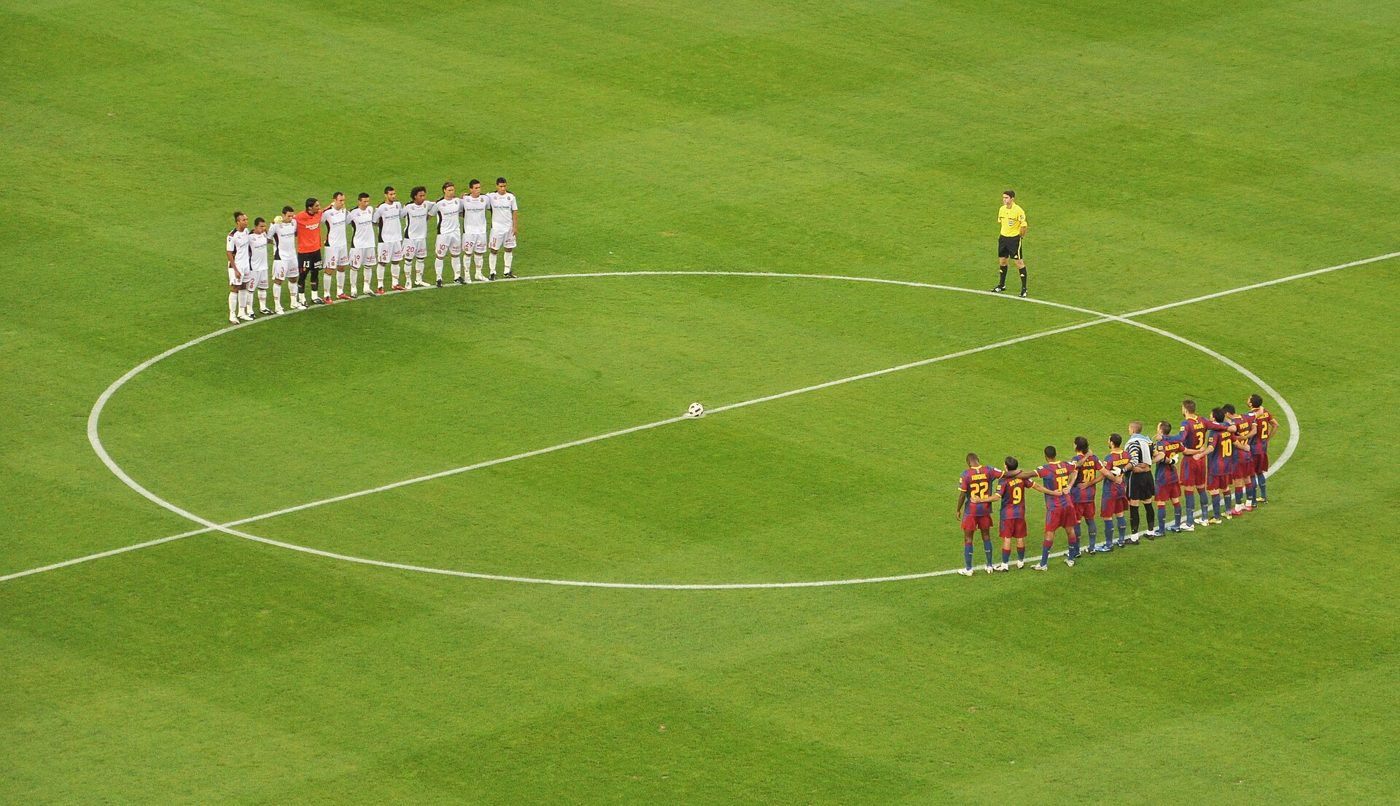
\includegraphics[width=0.78\textwidth,height=0.32\textheight,keepaspectratio]{../../resources/intros/PR-01-lets-do-some-sports.jpg}\\[0.4em]
{\footnotesize Image : Paolo Costa Baldi, CC BY-SA 3.0}
\end{center}

À regarder. Les vidéos sont un contexte. Elles ne sont pas le livrable.
\begin{itemize}
\item UX - Introduction \& Quest n°1, 01Edu \url{https://www.youtube.com/watch?v=UbE6WMeuvQg&list=PLHyAJ_GrRtf-RAtfngbRrFh1XDTnyXFDe}
\item UI - Introduction \& Quest n°1, 01Edu \url{https://www.youtube.com/watch?v=UbE6WMeuvQg&list=PLHyAJ_GrRtf-_aBft2jQL4-QAunn2bLvu}
\end{itemize}

\chapter{Exercice 00 : Projet 2 : Faisons du sport !}
\exnumber{00}
\extitle{Projet 2 : Faisons du sport !}
\exfiles{ex00/archive zip, nomme Name\_FirstName\_DeliverableName\_Date\_VersionNumber}
\exauthorize{Those named in the exercise}
\makeheaderfiles

Creation of a sports app with data tracking on mobile and e-watch (data visualization)

Yara is a runner. She runs 5 times a week and she's passionate! She'd like to challenge her own performance to make sure she is making progress.

Yara uses an Apple Watch and her iPhone.

'I wish I could have consistent data about my trainings, more than what already exists. I can run with my watch and I'd like to analyse and share my results with my sport coach."

She asks you to design an app on a watch and on mobile that could solve her problem.

You have to meet her after one week to give a first presentation of your work, after completing a tested mid-fidelity prototype.

The final presentation of your work will take place one week after the mid presentation, where you'll show a tested high-fidelity prototype.

\textbf{Durée estimée :} 2 semaines

\textbf{Team size}: 2

\textbf{Consignes :}

\begin{itemize}
\item Posez une stratégie UX et UI avant de foncer. Remettez le brief initial en question avec une recherche utilisateur.
\item Respectez les étapes : empathie, définir, énoncé du problème, idéation, prototype, test.
\item Vous devez interroger de vraies personnes pendant l'empathie, la recherche et les tests.
\item Déposez les documents sur Github, dans un zip nommé « ProjectTitle\_Name\_FirstName », et chaque livrable ainsi : « Name\_FirstName\_DeliverableName\_Date\_VersionNumber ». Exemple : « Doe\_John\_MidFiPrototype\_05242024\_V1 ».
\item Ajoutez un titre dans tous les documents écrits.
\item Soignez l'aspect global des livrables. Ils doivent être clairs, simples et lisibles. Vous pouvez regarder canva.com, sans surcharger le dessin de détails.
\item Dans les deux phases, testez vos prototypes avec au moins 5 personnes.
\item Make a presentation as if you were showing your work to Yara. Make sure there are at least 5 people in the audience.
\item Préparez un formulaire de retour pour le public. Il contient au moins les questions listées plus bas.
\item Dans les deux présentations, vous parlez à Barbara et à son équipe.
\item Durée : 10 minutes de présentation et 5 minutes de questions.
\item Vous pouvez vous servir des audits de présentation pour structurer vos présentations.
\item Amusez-vous !
\end{itemize}

\textbf{Outils :}

\begin{itemize}
\item Google Forms \url{https://docs.google.com/forms/u/0/}
\item Airtable \url{https://www.airtable.com/}
\item Typeform \url{https://www.typeform.com/}
\end{itemize}

\textbf{Pistes :}

\begin{itemize}
\item Effective presentation skills \url{https://academic.oup.com/femsle/article/364/24/fnx235/4587905}
\end{itemize}

Livrables intermédiaires :

\textbf{Citation :}

« Your mission in any presentation is to inform, educate, and inspire. » Robert Ballard

\medskip

\textbf{Phase 1 : audit de la présentation intermédiaire}

Vérifiez :

\begin{itemize}
\item Au moins 5 personnes assistent à la présentation
\item La présentation porte sur tout le processus UX, y compris :
\begin{itemize}
\item Le brief initial
\item Un planning, avec les phases UX, les outils choisis, le calendrier
\item Les résultats de la recherche utilisateur, qualitative et quantitative (persona, chiffres, etc.)
\item Un énoncé de problème qui ajuste le brief initial d'après la recherche
\item Une introduction du concept sorti de l'idéation
\item Le prototype moyenne fidélité animé (une vidéo de démo)
\item Les retours principaux du test d'utilisabilité
\item Les prochaines étapes du projet
\end{itemize}
\item La présentation ne dépasse pas 10 minutes
\item Les formulaires de retour ont été distribués au début de la présentation
\item Vous vous êtes amusés !
\end{itemize}

\medskip

\textbf{Phase 2 : audit de la présentation finale}

Vérifiez :

\begin{itemize}
\item Au moins 5 personnes assistent à la présentation
\item La présentation porte sur le processus UI, y compris :
\begin{itemize}
\item Un bref rappel de la présentation précédente
\item Un planning, avec les phases UI, les outils choisis, le calendrier
\item Une planche d'ambiance
\item Un styleguide (couleurs, marque, typographie, quelques éléments de la bibliothèque)
\item Le prototype haute fidélité animé (une vidéo de démo)
\item Les retours principaux des tests d'utilisabilité et de désirabilité
\item Les prochaines étapes du projet
\end{itemize}
\item La présentation ne dépasse pas 10 minutes
\item Les formulaires de retour ont été distribués au début de la présentation
\item Vous vous êtes amusés !
\end{itemize}

\textbf{Questions à poser dans les formulaires de retour}

\begin{itemize}
\item Que retenez-vous de cette présentation ?
\item De 0 à 10, le discours était-il clair ?
\item Pourquoi ?
\item De 0 à 10, la présentation était-elle engageante ?
\item Pourquoi ?
\item De 0 à 10, la présentation était-elle cohérente ?
\item Pourquoi ?
\item De 0 à 10, les visuels portaient-ils ?
\item Pourquoi ?
\item De 0 à 10, le problème était-il clair ?
\item Pourquoi ?
\item De 0 à 10, le prototype répond-il au problème ?
\item Pourquoi ?
\item Quelle recommandation feriez-vous pour améliorer cette présentation ?
\item Pourquoi ?
\end{itemize}


\chapter{Exercice 01 : Projet 2 : Faisons du sport !}
\exnumber{01}
\extitle{Projet 2 : Faisons du sport !}
\exfiles{ex01/archive zip, nomme Name\_FirstName\_DeliverableName\_Date\_VersionNumber}
\exauthorize{Ceux nommés dans l'exercice}
\makeheaderfiles

Montrez un prototype haute fidélité testé.

\textbf{Durée estimée :} 2 semaines

\textbf{Taille de l'équipe} : 2

\textbf{Consignes :}

\begin{itemize}
\item Testez vos prototypes avec au moins 5 personnes.
\item Faire une présentation comme si vous montriez votre travail à Yara. Assurez-vous qu'il y a au moins 5 personnes dans l'audience.
\item Déposez les documents sur Github, dans un zip nommé « ProjectTitle\_Name\_FirstName », et chaque livrable ainsi : « Name\_FirstName\_DeliverableName\_Date\_VersionNumber ». Exemple : « Doe\_John\_MidFiPrototype\_05242024\_V1 ».
\item Ajoutez un titre dans tous les documents écrits.
\item Soignez l'aspect global des livrables. Ils doivent être clairs, simples et lisibles. Vous pouvez regarder canva.com, sans surcharger le dessin de détails.
\item Préparez un formulaire de retour pour le public. Il contient au moins les questions listées plus bas.
\item Dans les deux présentations, vous parlez à Barbara et à son équipe.
\item Durée : 10 minutes de présentation et 5 minutes de questions.
\item Vous pouvez vous servir des audits de présentation pour structurer vos présentations.
\item Amusez-vous !
\end{itemize}

\textbf{Outils :}

\begin{itemize}
\item Google Forms \url{https://docs.google.com/forms/u/0/}
\item Airtable \url{https://www.airtable.com/}
\item Typeform \url{https://www.typeform.com/}
\end{itemize}

\textbf{Pistes :}

\begin{itemize}
\item Compétences de présentation efficaces \url{https://academic.oup.com/femsle/article/364/24/fnx235/4587905}
\end{itemize}

Livrables intermédiaires :

\textbf{Citation :}

« Your mission in any presentation is to inform, educate, and inspire. » Robert Ballard

\medskip

\textbf{Phase 1 : audit de la présentation intermédiaire}

Vérifiez :

\begin{itemize}
\item Au moins 5 personnes assistent à la présentation
\item La présentation porte sur tout le processus UX, y compris :
\begin{itemize}
\item Le brief initial
\item Un planning, avec les phases UX, les outils choisis, le calendrier
\item Les résultats de la recherche utilisateur, qualitative et quantitative (persona, chiffres, etc.)
\item Un énoncé de problème qui ajuste le brief initial d'après la recherche
\item Une introduction du concept sorti de l'idéation
\item Le prototype moyenne fidélité animé (une vidéo de démo)
\item Les retours principaux du test d'utilisabilité
\item Les prochaines étapes du projet
\end{itemize}
\item La présentation ne dépasse pas 10 minutes
\item Les formulaires de retour ont été distribués au début de la présentation
\item Vous vous êtes amusés !
\end{itemize}

\medskip

\textbf{Phase 2 : audit de la présentation finale}

Vérifiez :

\begin{itemize}
\item Au moins 5 personnes assistent à la présentation
\item La présentation porte sur le processus UI, y compris :
\begin{itemize}
\item Un bref rappel de la présentation précédente
\item Un planning, avec les phases UI, les outils choisis, le calendrier
\item Une planche d'ambiance
\item Un styleguide (couleurs, marque, typographie, quelques éléments de la bibliothèque)
\item Le prototype haute fidélité animé (une vidéo de démo)
\item Les retours principaux des tests d'utilisabilité et de désirabilité
\item Les prochaines étapes du projet
\end{itemize}
\item La présentation ne dépasse pas 10 minutes
\item Les formulaires de retour ont été distribués au début de la présentation
\item Vous vous êtes amusés !
\end{itemize}

\textbf{Questions à poser dans les formulaires de retour}

\begin{itemize}
\item Que retenez-vous de cette présentation ?
\item De 0 à 10, le discours était-il clair ?
\item Pourquoi ?
\item De 0 à 10, la présentation était-elle engageante ?
\item Pourquoi ?
\item De 0 à 10, la présentation était-elle cohérente ?
\item Pourquoi ?
\item De 0 à 10, les visuels portaient-ils ?
\item Pourquoi ?
\item De 0 à 10, le problème était-il clair ?
\item Pourquoi ?
\item De 0 à 10, le prototype répond-il au problème ?
\item Pourquoi ?
\item Quelle recommandation feriez-vous pour améliorer cette présentation ?
\item Pourquoi ?
\end{itemize}


\end{document}
